\begin{infocard}{Polígono regular}
    \begin{wrapfigure}{r}{0.32\linewidth}
        \centering
        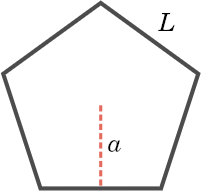
\includegraphics[width=\linewidth]{../images/apotema.png}
    \end{wrapfigure}
    Si un polígono regular de $n$ lados, de longitud $L$, un perímetro de $P$
    unidades, un apotema de $a$ unidades, entonces el área $A$ en unidades
    cuadradas es:
    \[A=\dfrac{nLa}{2}\]
    donde el perímetro es $P=nL$.\\
\end{infocard}